\subsection{问题一的模型建立与求解}

\subsubsection{交会定位区域的几何模型}

记第 $i$ 个检测点的二维位置坐标为 $S_i=(x_i,y_i)\in\mathbb{R}^2$，该检测点测得的示向度为 $\theta_i$。由题设，真实方位角位于 $\theta_i$ 左右各 $\delta=1^\circ$ 的范围内。以位置 $S_i$ 为顶点、两条向前无限延伸的误差边界射线为边界所夹的闭角区域记为 $C_i$。根据交会定位法，与全部观测相容的干扰源位置必须同时属于所有 $C_i$，故定位区域为
\begin{equation}
  \Omega=\bigcap_{i=1}^{n}C_i.
  \label{eq:q1-intersection}
\end{equation}

由于角区宽度 $2\delta<180^\circ$，每个 $C_i$ 是两个闭半平面的交，故非空、有界且具有非零面积的
$\Omega$ 为凸多边形。保留满足全部观测约束的边界交点并取凸包，可得逆时针排列的顶点
$V_1,\ldots,V_m$，即

\begin{equation}
  \Omega=\operatorname{conv}\{V_1,V_2,\ldots,V_m\},
  \label{eq:q1-convex-hull}
\end{equation}

其中 $\operatorname{conv}$ 表示凸包。边界交点仍须逐一检查是否处于全部前向误差角区内，
保留的顶点用于后续直径和圆覆盖计算。

图~\ref{fig:q1-region-intersection} 给出了两个角度误差区域交会形成有界凸定位区域的示意。

\begin{figure}[H]
  \centering
  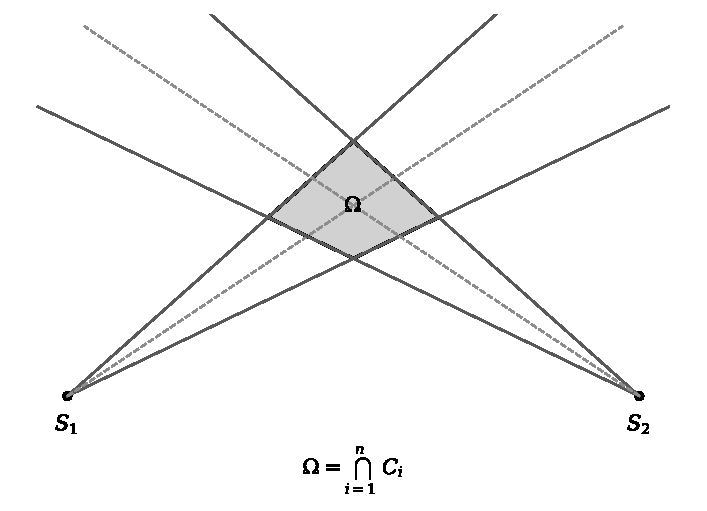
\includegraphics[width=0.58\textwidth]{figures/q1-region-intersection.pdf}
  \caption{多个示向度误差区域的公共交集（角度不按比例）}
  \label{fig:q1-region-intersection}
\end{figure}

\subsubsection{定位区域直径及其求解}

按照题目定义，定位区域的直径为区域内任意两点距离的最大值，即
\begin{equation}
  D=\max_{P,Q\in\Omega}d(P,Q)
   =\max_{P,Q\in\Omega}\|P-Q\|_2.
  \label{eq:q1-diameter-definition}
\end{equation}

由于定位区域闭且有界，距离最大值能够取得。

\noindent\textbf{命题 1：}{\kaishu 凸多边形的直径必由其两个顶点取得，即}
\begin{equation}
  D=\max_{1\leq i,j\leq m}\|V_i-V_j\|_2.
  \label{eq:q1-vertex-diameter}
\end{equation}

\noindent\textbf{证明：}
任取 $P,Q\in\Omega$，写成顶点的凸组合 $P=\sum_i\lambda_iV_i$、$Q=\sum_j\mu_jV_j$，其中系数非负且各自之和为 $1$。由三角不等式，
\begin{equation}
  \|P-Q\|_2
  =\left\|\sum_{i,j}\lambda_i\mu_j(V_i-V_j)\right\|_2
  \leq\max_{i,j}\|V_i-V_j\|_2.
  \label{eq:q1-diameter-proof}
\end{equation}

由于 $\sum_{i,j}\lambda_i\mu_j=1$ 且顶点属于 $\Omega$，任意两点距离不超过最大顶点对距离，
而最远顶点对取得该上界。\hfill$\square$

本文采用旋转卡壳法求解最远顶点对。由旋转卡壳定理~\cite{toussaint1983}，直径端点必属于对踵点对。
对边向量 $E_i=V_{i+1}-V_i$，以
$A(i,j)=|E_i\mathbin{\boldsymbol{\times}}(V_j-V_i)|$ 衡量顶点到该边所在直线的距离；
依次增加 $j$ 至该量不再增大，相等时同时检查两个候选点。两个指标均至多绕多边形一周，
故时间复杂度为 $O(m)$。

\subsubsection{直径圆的覆盖判据}

设旋转卡壳法得到的一组直径端点为 $V_p,V_q$。以线段 $V_pV_q$ 为直径构造圆，下文所称“圆覆盖”均指该圆的闭圆面覆盖。其圆心和半径分别为
\begin{equation}
  O=\frac{V_p+V_q}{2},\qquad r=\frac{D}{2}.
  \label{eq:q1-diameter-circle}
\end{equation}

\noindent\textbf{命题 2：}{\kaishu 直径圆能够覆盖整个定位区域 $\Omega$ 的充分必要条件为}
\begin{equation}
  \max_{1\leq j\leq m}\|V_j-O\|_2\leq\frac{D}{2}.
  \label{eq:q1-circle-criterion}
\end{equation}

\noindent\textbf{证明：}
若圆覆盖区域，必然包含全部顶点；反之，闭圆盘为凸集，包含全部顶点就包含它们的凸包 $\Omega$。\hfill$\square$

直径圆不一定覆盖第三个顶点，如图~\ref{fig:q1-diameter-circle} 所示，因此仍须逐顶点检查
式~\eqref{eq:q1-circle-criterion}；问题二据此改用最小包围圆衡量定位不确定性。

\begin{figure}[H]
  \centering
  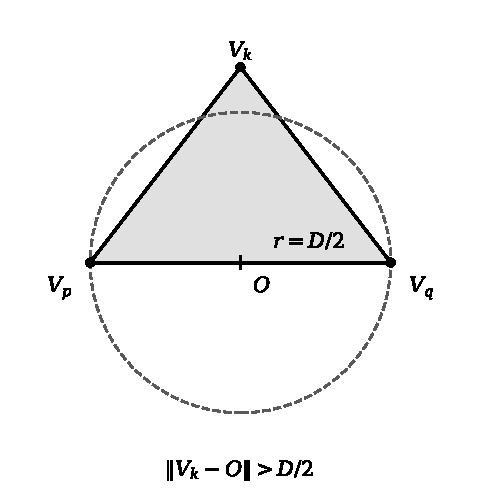
\includegraphics[width=0.52\textwidth]{figures/q1-diameter-circle.pdf}
  \caption{直径圆未覆盖定位区域的反例（长度不按比例）}
  \label{fig:q1-diameter-circle}
\end{figure}

求解过程依次为：求交会多边形、用旋转卡壳计算直径、逐顶点检验直径圆覆盖性。

\subsubsection{建模边界及对后续问题的影响}

问题一按题意求纯角度交会区域 $\Omega$。进一步利用目标圆形区域和成功接收时距离不超过 $1500\ \mathrm m$ 的条件，可得更小的物理可行域

\begin{equation}
  K=\Omega\cap\overline B(O_0,1800)
  \cap\bigcap_{i=1}^{n}\overline B(S_i,1500).
  \label{eq:q1-physical-region}
\end{equation}

其中 $1500\ \mathrm m$ 是有效接收半径的统一上界，$1000\ \mathrm m$ 不构成源与测点间的距离下界。
$K$ 仍为凸集，但圆盘可能截断 $\Omega$ 并形成图~\ref{fig:q1-curved-regions} 所示的圆弧边界。

\begin{figure}[H]
  \centering
  \begin{subfigure}[t]{0.48\textwidth}
    \centering
    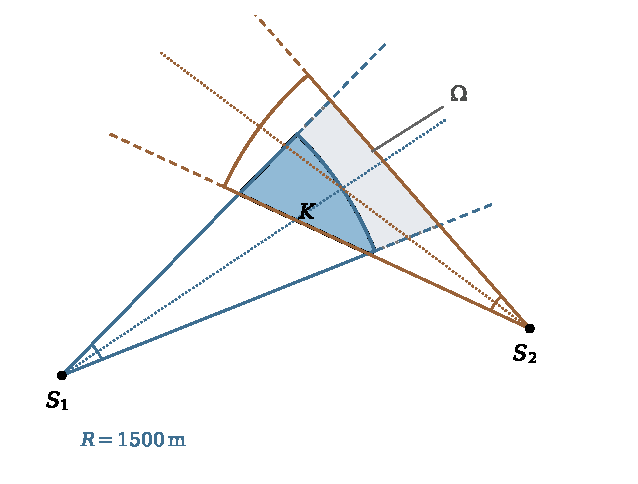
\includegraphics[width=\linewidth]{figures/q1-receive-radius-arc.pdf}
    \caption{两个有限探测扇形交会形成圆弧边界}
  \end{subfigure}\hfill
  \begin{subfigure}[t]{0.48\textwidth}
    \centering
    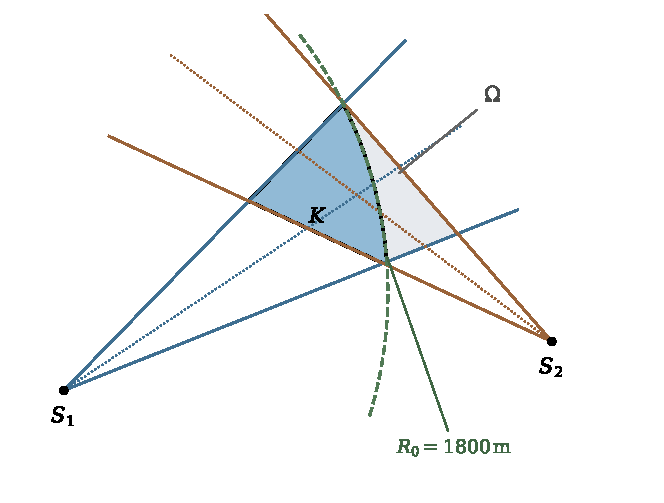
\includegraphics[width=\linewidth]{figures/q1-arena-radius-arc.pdf}
    \caption{目标圆形区域截断交会多边形}
  \end{subfigure}
  \caption{定位区域出现圆弧边界的两种情形（图中长度不按比例）}
  \label{fig:q1-curved-regions}
\end{figure}

圆弧上的直径端点可能不在直线边界交点中。由 $K\subseteq\Omega$，问题一的多边形直径仍是物理
可行域直径的上界。问题二用固定边数的外切正多边形替代圆盘，得到
$K\subseteq\widehat K$ 及
$\operatorname{diam}(K)\leq\operatorname{diam}(\widehat K)$；该外近似保留真实位置并提供保守覆盖判定。
